\documentclass[crop,tikz]{standalone}
\usepackage[utf8]{inputenc}
\usepackage{tikz}
\usepackage{pgfplots}
\usepackage{bm}
\pgfplotsset{compat=newest}
\usepgfplotslibrary{groupplots}
\begin{document}
% This file was created by tikzplotlib v0.8.2.
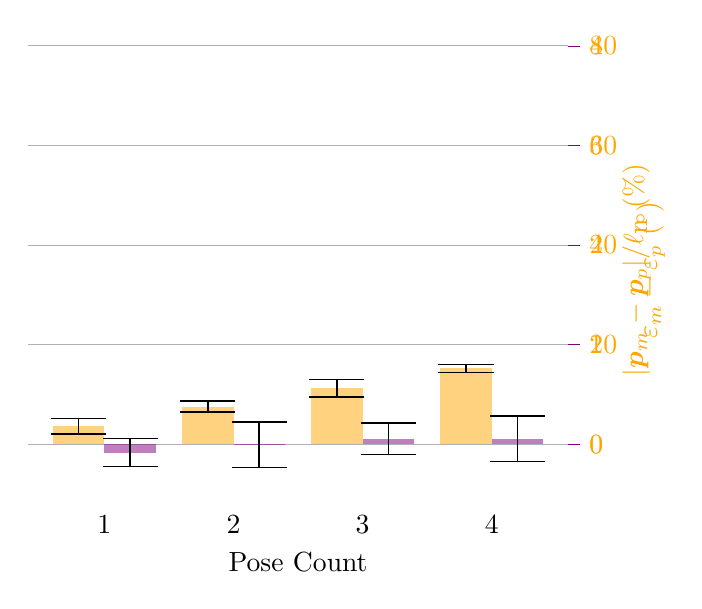
\begin{tikzpicture}
\definecolor{color0}{rgb}{1,0.647058823529412,0}
\definecolor{color1}{rgb}{0.501960784313725,0,0.501960784313725}
\begin{axis}[
anchor=origin,
axis line style={draw=none},
tick align=outside,
tick pos=both,
x grid style={white!69.01960784313725!black},
xmin=-0.59, xmax=3.59,
xtick style={color=black},
xtick style={draw=none},
xtick={0,1,2,3},
xticklabels={ , , , },
y grid style={white!69.01960784313725!black},
ylabel style={color=color0},
ylabel={\(\displaystyle |\bm{p}_m - \bm{p}_p|/\ell_{\textnormal{n}}\) (\%)},
ymin=-0.5, ymax=4,
ytick pos=left,
ytick pos=right,
ytick style={color=color0},
ytick style={color=color0},
yticklabel style={color=color0}
]
\draw[fill=color0,draw opacity=0,fill opacity=0.5] (axis cs:0,0) rectangle (axis cs:-0.4,0.182005140998015);
\draw[fill=color0,draw opacity=0,fill opacity=0.5] (axis cs:1,0) rectangle (axis cs:0.6,0.376934216956995);
\draw[fill=color0,draw opacity=0,fill opacity=0.5] (axis cs:2,0) rectangle (axis cs:1.6,0.56218185103056);
\draw[fill=color0,draw opacity=0,fill opacity=0.5] (axis cs:3,0) rectangle (axis cs:2.6,0.761494465856718);
\path [draw=black, semithick]
(axis cs:-0.2,0.103783119023693)
--(axis cs:-0.2,0.260227162972336);
\path [draw=black, semithick]
(axis cs:0.8,0.321160265085024)
--(axis cs:0.8,0.432708168828965);
\path [draw=black, semithick]
(axis cs:1.8,0.474943802907275)
--(axis cs:1.8,0.649419899153845);
\path [draw=black, semithick]
(axis cs:2.8,0.721622963294239)
--(axis cs:2.8,0.801365968419196);
\addplot [semithick, black, mark=-, mark size=10, mark options={solid}, only marks]
table {%
-0.2 0.103783119023693
0.8 0.321160265085024
1.8 0.474943802907275
2.8 0.721622963294239
};
\addplot [semithick, black, mark=-, mark size=10, mark options={solid}, only marks]
table {%
-0.2 0.260227162972336
0.8 0.432708168828965
1.8 0.649419899153845
2.8 0.801365968419196
};
\end{axis}
\begin{axis}[
anchor=origin,
axis line style={draw=none},
axis y line=right,
tick align=outside,
tick pos=both,
x grid style={white!69.01960784313725!black},
xlabel={Pose Count},
xmin=-0.59, xmax=3.59,
xtick style={color=black},
xtick style={draw=none},
xtick={0,1,2,3},
xticklabels={1,2,3,4},
y grid style={white!69.01960784313725!black},
ylabel style={color=color0},
ylabel={\(\displaystyle \varepsilon_m - \varepsilon_p\) (\(\displaystyle ^\circ\))},
ymajorgrids,
ymin=-10, ymax=80,
ytick pos=left,
ytick pos=right,
ytick style={color=color0},
ytick style={color=color1},
yticklabel style={color=color0}
]
\draw[fill=color1,draw opacity=0,fill opacity=0.5] (axis cs:0,0) rectangle (axis cs:0.4,-1.65422862933917);
\draw[fill=color1,draw opacity=0,fill opacity=0.5] (axis cs:1,0) rectangle (axis cs:1.4,-0.0920250465413801);
\draw[fill=color1,draw opacity=0,fill opacity=0.5] (axis cs:2,0) rectangle (axis cs:2.4,1.09881957299751);
\draw[fill=color1,draw opacity=0,fill opacity=0.5] (axis cs:3,0) rectangle (axis cs:3.4,1.10361241557092);
\path [draw=black, semithick]
(axis cs:0.2,1.14627344804069)
--(axis cs:0.2,-4.45473070671903);
\path [draw=black, semithick]
(axis cs:1.2,4.49310558845599)
--(axis cs:1.2,-4.67715568153875);
\path [draw=black, semithick]
(axis cs:2.2,4.22604537450781)
--(axis cs:2.2,-2.02840622851278);
\path [draw=black, semithick]
(axis cs:3.2,5.69166635776884)
--(axis cs:3.2,-3.48444152662699);
\addplot [semithick, black, mark=-, mark size=10, mark options={solid}, only marks]
table {%
0.2 1.14627344804069
1.2 4.49310558845599
2.2 4.22604537450781
3.2 5.69166635776884
};
\addplot [semithick, black, mark=-, mark size=10, mark options={solid}, only marks]
table {%
0.2 -4.45473070671903
1.2 -4.67715568153875
2.2 -2.02840622851278
3.2 -3.48444152662699
};
\end{axis}
\end{tikzpicture}
%% End matplotlib2tikz content %% 
\end{document}